\section{Resultado dos Cenários de Teste}

Após a apuração dos cenários descritos acima, chegamos aos seguintes resultados por serviço:

\begin{center}
	% TABELAS DE CASES DE TEST
	TABELAS PENDENTES :D		
\end{center}


\section{Apresentação dos Resultados Obtidos}

Levando em consideração os resultados obtidos através da aplicação de todos os cenários de testes descritos acima sob os serviços desenvolvidos neste trabalho, observando os percentuais atingidos com base na média descrita dos principais Serviços do Atendimento ao Público, notamos que a solução proposta é capaz de reduzir em até 20,46\%, dos registros de atendimentos diários, conforme visto abaixo na figura 22:	


\begin{figure}[!htb]
	\centering
	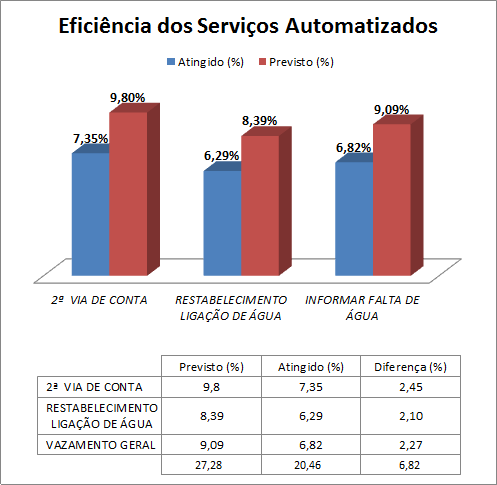
\includegraphics{figuras/eficiencia_servicos.png}
	\caption{Gráfico de avaliação dos serviços automatizados}	
	Fonte - Autoria Própria
\end{figure}

